\documentclass[11pt,a4paper]{article}
\usepackage[utf8]{inputenc}
\usepackage[francais]{babel}
\usepackage[T1]{fontenc}
\usepackage{amsmath}
\usepackage{amsfonts}
\usepackage{amssymb}
\usepackage{hyperref}
\usepackage{graphicx}

\title{Projet d'option GSI Vivaldi \\ Book de passation}
\author{Nicolas Joseph, Raphaël Gaschignard\\ Guillaume Blondeau, Cyprien Quilici, Jacob Tardieu}

\begin{document}
\maketitle

\section{Présentation}



\section{Architecture globale}

\begin{figure}[h]
   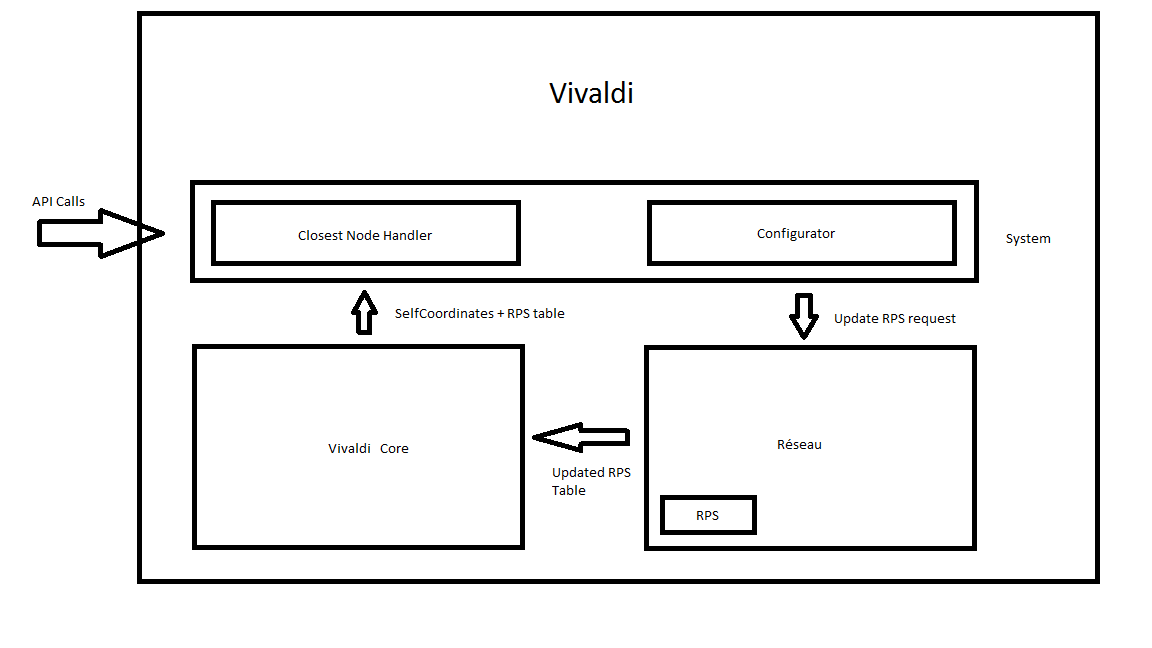
\includegraphics[scale=0.4]{VivaldiArchitecture}
   \caption{\label{acteur} Modèle Acteur}
\end{figure}

Le projet est divisé en trois principaux acteurs : 
\begin{itemize}
	\item[$\bullet$] VivaldiActor : Cet acteur est la brique principale du projet. Il s'occupe de créer les deux autres acteurs. Il détient les schedulers qui déclenchent les appels vers l'acteur Communication. Il gère aussi le tableau des closes nodes.
	\item[$\bullet$] Communication : 
		\begin{itemize}
			\item Cet acteur s'occupe de l'appeler chaque n\oe ud dans le tableau des RPS afin s'obtenir la position de chacun. Il envoie à la fin ce tableau à l'acteur ComputingAlgorithm pour appliquer Vivaldi.
			\item Il s'occupe aussi de recevoir les appels "ping" des autres n\oe uds et de leur répondre.
		\end{itemize}
		Dans les deux situations, l'acteur en profite pour enrichir ses RPS : il prend ses contacts et ceux de ses contacts et les mixe pour créer un nouveau tableau de RPS.
	\item[$\bullet$] ComputingAlgorithm : Cet acteur implémente l'algorithme Vivaldi. Il calcule les nouvelles coordonnées du n\oe ud et les renvoie avec les RPS au VivaldiActor.
\end{itemize}

\section{Points d'amélioration}



\end{document}